\index{general}{Advection-Diffusion Equation}

We start with the 1D advection-diffusion equation
\begin{equation}
\rho C_p \left( \frac{\partial T}{\partial t} 
+ u \frac{\partial T}{\partial x}
\right)
= \frac{\partial }{\partial x} \left( k \frac{\partial T}{\partial x}  \right)
+H
\end{equation}
This is the {\color{olive}strong form} of the ODE to solve.
As in the previous section, I multiply this equation by a function $f(x)$ and integrate it over 
the domain $\Omega$:
\[
\int_{\Omega} f(x)  \rho C_p\frac{\partial T}{\partial t} dx
+
\int_{\Omega} f(x)  \rho C_p u \frac{\partial T}{\partial x} dx
\!=\!
\int_{\Omega} f(x) \frac{\partial }{\partial x}\! \left(\! k\! \frac{\partial T}{\partial x}\!  \right)\! dx
+
\int_{\Omega} f(x) H dx 
\]
As in the previous section I integrate the r.h.s. by parts:
\[
\int_{\Omega} f(x) \frac{\partial }{\partial x} \left( k \frac{\partial T}{\partial x}  \right) dx
=
\left[
f(x) k \frac{\partial T}{\partial x}
\right]_{\partial \Omega}
-
\int_{\Omega} \frac{\partial f}{\partial x}  k \frac{\partial T}{\partial x}  dx
\]
Disregarding the boundary term for now, 
we then obtain the {\color{olive}weak form} of the diffusion equation in 1D:
\[
\boxed{
\int_{\Omega} f(x) \rho C_p \frac{\partial T}{\partial t} dx
+
\int_{\Omega} f(x)  \rho C_p u \frac{\partial T}{\partial x} dx
+
\int_{\Omega} \frac{\partial f}{\partial x}  k \frac{\partial T}{\partial x}  dx = 
\int_{\Omega} f(x) H dx 
}
\]

We then use the additive property of the integral $\int_\Omega \dots = \sum_{elts} \int_{\Omega_e} \dots$
\[
\sum_{elts} \left(     
\underbrace{ \int_{\Omega_e} f(x) \rho C_p   \frac{\partial T}{\partial t} dx }_{{\Lambda}_f^e}
+
\underbrace{  \int_{\Omega_e} f(x)  \rho C_p u \frac{\partial T}{\partial x} dx  }_{{\Sigma}_f^e}
+
\underbrace{\int_{\Omega_e} \frac{\partial f}{\partial x}  k \frac{\partial T}{\partial x}  dx}_{{\Upsilon}_f^e}    
- 
\underbrace{\int_{\Omega_e} f(x) H dx }_{{\Omega}_f^e}
  \right) = 0  
\]

In the element, we have seen that the temperature can be written:

\[
T^h(x) 
= {\color{Violet}N}^\theta_{k}(x) T_k + {\color{Violet}N}^\theta_{k+1}(x) T_{k+1}  
\]
In the previous presentation we have computed  ${\Lambda}_f^e$ and ${\Upsilon}_f^e$.
Let us now turn to ${\Sigma}_f^e$ and ${\Omega}_f^e$.

\begin{eqnarray}
{\Sigma}_f^e 
&=&\int_{x_k}^{x_{k+1}} f(x) \rho C_p u\frac{\partial T^h}{\partial x} dx \nn\\
&=&\int_{x_k}^{x_{k+1}} f(x) \rho C_p u\frac{\partial 
[ {\color{Violet}N}_{k}^\theta(x) {T}_k + {\color{Violet}N}_{k+1}^\theta(x) {T}_{k+1} ] }{\partial x} dx \nn\\
&=&\int_{x_k}^{x_{k+1}} f(x) \rho C_p u\frac{\partial  {\color{Violet}N}_{k}^\theta }{\partial x} T_k dx 
+  \int_{x_k}^{x_{k+1}} f(x) \rho C_p u\frac{\partial  {\color{Violet}N}_{k+1}^\theta }{\partial x} T_{k+1} dx \nn\\
&=& \left(  \int_{x_k}^{x_{k+1}} f(x) \rho C_p u\frac{\partial  {\color{Violet}N}_{k}^\theta }{\partial x} dx \right) T_k 
+ \left( \int_{x_k}^{x_{k+1}} f(x) \rho C_p u\frac{\partial  {\color{Violet}N}_{k+1}^\theta }{\partial x} dx \right)T_{k+1}  \nn
%&=&  \int_{x_k}^{x_{k+1}} {\color{blue}f}(x) \rho C_p \;\;  [ {\color{blue}N}_{k}(x) \dot{T}_k + {\color{blue}N}_{k+1}(x) \dot{T}_{k+1} ] \;\; dx  \nn\\
%&=&  \int_{x_k}^{x_{k+1}} {\color{blue}f}(x) \rho C_p {\color{blue}N}_{k}(x) \dot{T}_k  dx  + \int_{x_k}^{x_{k+1}} {\color{blue}f}(x) \rho C_p {\color{blue}N}_{k+1}(x) \dot{T}_{k+1}   dx \nn\\
%&=&  \left( \int_{x_k}^{x_{k+1}} {\color{blue}f}(x) \rho C_p  {\color{blue}N}_{k}(x) dx \right) \dot{T}_k  
%+ \left( \int_{x_k}^{x_{k+1}} {\color{blue}f}(x) \rho C_p {\color{blue}N}_{k+1}(x) dx \right)  \dot{T}_{k+1}  \nn
\end{eqnarray}

Taking ${\color{Violet}f}(x)={\color{Violet}N}_k^\theta(x)$ and omitting '$(x)$' in the rhs:
\[
{\Sigma}_{N_k^\theta}^e=
\left( \int_{x_k}^{x_{k+1}} \rho C_p u {\color{Violet}N}_k^\theta \frac{\partial  {\color{Violet}N}_{k}^\theta }{\partial x} dx \right) T_k 
+ 
\left( \int_{x_k}^{x_{k+1}} \rho C_p u {\color{Violet}N}_k^\theta \frac{\partial  {\color{Violet}N}_{k+1}^\theta }{\partial x} dx \right)T_{k+1}  \nn
\]
Taking ${\color{Violet}f}(x)={\color{Violet}N}_{k+1}^\theta(x)$ and omitting '$(x)$' in the rhs:
\[
{\Sigma}_{N_{k+1}^\theta}^e=
\left( \int_{x_k}^{x_{k+1}} \rho C_p u {\color{Violet}N}_{k+1}^\theta \frac{\partial  {\color{Violet}N}_{k}^\theta }{\partial x} dx \right) T_k + 
\left( \int_{x_k}^{x_{k+1}} \rho C_p u {\color{Violet}N}_{k+1}^\theta \frac{\partial  {\color{Violet}N}_{k+1}^\theta }{\partial x} dx \right)T_{k+1}  \nn
\]



\[
\left(
\begin{array}{c}
{\Sigma}_{N_k^\theta}  \\ \\ {\Sigma}_{N_{k+1}^\theta}
\end{array}
\right)
\!=\!
\left(
\begin{array}{cc}
\int_{x_k}^{x_{k+1}} \rho C_p u {\color{Violet}N}_k^\theta \frac{\partial      {\color{Violet}N}_{k}^\theta }{\partial x} dx  & 
\int_{x_k}^{x_{k+1}} \rho C_p u {\color{Violet}N}_k^\theta \frac{\partial      {\color{Violet}N}_{k+1}^\theta }{\partial x} dx \\ \\
\int_{x_k}^{x_{k+1}} \rho C_p u {\color{Violet}N}_{k+1}^\theta \frac{\partial  {\color{Violet}N}_{k}^\theta }{\partial x} dx  & 
\int_{x_k}^{x_{k+1}} \rho C_p u {\color{Violet}N}_{k+1}^\theta \frac{\partial  {\color{Violet}N}_{k+1}^\theta }{\partial x} dx 
\end{array}
\right)
\!\cdot\!
\left(
\begin{array}{c}
{T}_k \\ \\
{T}_{k+1}
\end{array}
\right)
\]
or,
\[
\left(
\begin{array}{c}
{\Sigma}_{N_k^\theta} \\ \\ {\Sigma}_{N_{k+1}^\theta}
\end{array}
\right)
\!=\!
\left[
\int_{x_k}^{x_{k+1}}
\rho C_p u
\left(
\begin{array}{cc}
{\color{Violet}N}_k^\theta \frac{\partial     {\color{Violet}N}_{k}^\theta }{\partial x}   & 
{\color{Violet}N}_k^\theta \frac{\partial     {\color{Violet}N}_{k+1}^\theta }{\partial x}  \\ \\
{\color{Violet}N}_{k+1}^\theta \frac{\partial {\color{Violet}N}_{k}^\theta }{\partial x}   & 
{\color{Violet}N}_{k+1}^\theta \frac{\partial {\color{Violet}N}_{k+1}^\theta }{\partial x} 
\end{array}
\right)
dx
\right]
\cdot
\left(
\begin{array}{c}
{T}_k \\ \\ 
{T}_{k+1}
\end{array}
\right)
\]

Finally, we have already defined the vectors 
\[
{\vec N}^T = 
\left(
\begin{array}{c}
{\color{Violet}N}_k^\theta(x)  \\ \\  {\color{Violet}N}_{k+1}^\theta (x)
\end{array}
\right)
\quad\quad
{\vec B}^T=
\left(
\begin{array}{cc}
 \frac{\partial {\color{Violet}N}_k^\theta}{\partial x}   \\ \\
 \frac{\partial {\color{Violet}N}_{k+1}^\theta}{\partial x}
\end{array}
\right)
\quad
\quad
{\vec T}^e = 
\left(
\begin{array}{c}
T_k \\ \\ T_{k+1}
\end{array}
\right)
\]
so that 
\[
\left(
\begin{array}{c}
{\Sigma}_{N_k^\theta} \\  \\ {\Sigma}_{N_{k+1}^\theta}
\end{array}
\right)
=
\left( \int_{x_k}^{x_{k+1}}   {\vec {\color{Violet}N}}^T \rho C_p u {\vec {\color{Violet}B}} dx  \right) \cdot {\vec T}^e
= {\bm K}_a \cdot \vec T^e
\]
One can easily show that 
\[
{\bm K}_a^e=
\rho C_p u
\left(
\begin{array}{cc}
-1/2 & 1/2 \\ \\
-1/2 & 1/2 
\end{array}
\right)
\]
Note that the matrix ${\bm K}_a^e$ is {\sl not} symmetric. 

Let us now look at the source term:
\begin{eqnarray}
{\Omega}_f^e &=&
\int_{x_k}^{x^{k+1}} f(x) H(x) dx \nn
\end{eqnarray}
Taking ${\color{Violet}f}(x)={\color{Violet}N}_k^\theta(x)$: 
\[
{\Omega}_{N_k^\theta}=
\int_{x_k}^{x^{k+1}} {\color{Violet}N}_k^\theta(x) H(x) dx \nn
\]
Taking ${\color{Violet}f}(x)={\color{Violet}N}_{k+1}^\theta(x)$: 
\[
{\Omega}_{N_{k+1}^\theta}=
\int_{x_k}^{x^{k+1}} {\color{Violet}N}_{k+1}^\theta(x) H(x) dx \nn
\]
We can rearrange both equations as follows:
\[
\left(
\begin{array}{cc}
 {\Omega}_{N_k^\theta} \\ \\ {\Omega}_{N_{k+1}^\theta}
\end{array}
\right)
=
\left(
\begin{array}{cc}
\int_{x_k}^{x^{k+1}} {\color{Violet}N}_k^\theta(x) H(x) dx \nn \\ \\ 
\int_{x_k}^{x^{k+1}} {\color{Violet}N}_{k+1}^\theta(x) H(x) dx \nn
\end{array}
\right)
\]
or,
\[
\left(
\begin{array}{cc}
 {\Omega}_{N_k^\theta} \\ \\ {\Omega}_{N_{k+1}^\theta}
\end{array}
\right)
=
\int_{x_k}^{x^{k+1}}
\left(
\begin{array}{cc}
{\color{Violet}N}_k^\theta(x)  H(x)  \nn \\ \\ 
{\color{Violet}N}_{k+1}^\theta(x) H(x)  \nn
\end{array}
\right)
dx
=
\left(
\int_{x_k}^{x^{k+1}}
{\vec {\color{Violet}N}}^T H(x) dx
\right)
\]


The weak form discretised over 1 element becomes
\begin{eqnarray}
&&\underbrace{\left( \int_{x_k}^{x_{k+1}}   {\vec {\color{Violet}N}}^T \rho C_p {\vec {\color{Violet}N}} dx  \right) }_{\bm M^e} \cdot \dot{\vec T}^e
+
\underbrace{\left( \int_{x_k}^{x_{k+1}}   {\vec {\color{Violet}N}}^T \rho C_p u {\vec {\color{Violet}B}} dx  \right)}_{{\bm K}_a^e} \cdot {\vec T}^e 
 +
\underbrace{\left( \int_{x_k}^{x_{k+1}}   {\vec {\color{Violet}B}}^T k {\vec {\color{Violet}B}} dx  \right)}_{{\bm K}_d^e} \cdot {\vec T}^e 
=
\underbrace{\left( \int_{x_k}^{x_{k+1}}   {\vec {\color{Violet}N}}^T H(x) dx \right)}_{{\vec F}^e} \nn 
\end{eqnarray}
or,
\[
\boxed{
{\bm M}^e \cdot \dot{\vec T}^e + ({\bm K}_d^e + {\bm K}_a^e)\cdot {\vec T}^e = {\vec F}^e
}
\]
or,
\[
\boxed{
{\bm M}^e \cdot \frac{\partial {\vec T}^e}{\partial t} + ({\bm K}_a^e + {\bm K}_d^e) \cdot {\vec T}^e = {\vec F}^e
}
\]

As in the diffusion case of the previous section these matrices and vectors will need to be 
assembled into ${\bm M}$, ${\bm K}_a$, ${\bm K}_d$, $\vec{T}$ and $\vec{F}$:
\[
{\bm M} \cdot \frac{\partial {\vec T}}{\partial t} + ({\bm K}_a + {\bm K}_d) \cdot {\vec T} = {\vec F}
\]

We can revisit the time discretisation again, assuming for simplicity that the coefficients of the PDE are not time-dependent.
Choosing a fully explicit approach would have us write
\[
{\bm M} \cdot \frac{{\vec T}^{n+1}-{\vec T}^n}{\delta t} + ({\bm K}_a + {\bm K}_d) \cdot {\vec T}^{n} = {\vec F}
\quad
\Rightarrow
\quad
{\bm M} \cdot {\vec T}^{n+1} = [{\bm M} - ({\bm K}_a + {\bm K}_d) \delta t] \cdot {\vec T}^{n} = {\vec F}
\]
while choosing a fully implicit approach would have us write
\[
{\bm M} \cdot \frac{{\vec T}^{n+1}-{\vec T}^n}{\delta t} + ({\bm K}_a + {\bm K}_d) \cdot {\vec T}^{n+1} = {\vec F}
\quad
\Rightarrow
\quad
[{\bm M} +  ({\bm K}_a + {\bm K}_d) \delta t] \cdot {\vec T}^{n+1}
={\bm M}\cdot {\vec T}^n+ {\vec F} \delta t
\]
We can also consider a more generic approach and write:
\[
{\bm M} \cdot \frac{{\vec T}^{n+1}-{\vec T}^n}{\delta t} + ({\bm K}_a + {\bm K}_d) \cdot (\alpha {\vec T}^{n+1}+(1-\alpha)\vec{T}^{n}) = {\vec F}
\]
\[
[{\bm M} +  \alpha({\bm K}_a + {\bm K}_d) \delta t] \cdot {\vec T}^{n+1}
=
[{\bm M} - (1-\alpha)({\bm K}_a + {\bm K}_d) \delta t] \cdot {\vec T}^{n} + {\vec F}\delta t
\]
When $\alpha=0$ we recover the explicit scheme, when $\alpha=1$ we recover the implicit one, and when $\alpha=1/2$ we get a so-called 
mid-point algorithm (Crank-Nicolson).

Write about SUPG!!!

%-/-/-/-/-/-/-/-/-/-/-/-/-/-/-/-/-/-/-/
\begin{center}
\begin{minipage}[t]{0.77\textwidth}
\par\noindent\rule{\textwidth}{0.4pt}

\begin{center}

\includegraphics[width=0.8cm]{images/garftr} \\
{\color{orange}Exercise FEM-2}
\end{center}

Let us consider the domain $[0,1]$. The temperature field at $t=0$ is 
given by $T=1$ for $x<0.25$ and $T=0$ otherwise. The prescribed 
velocity is $u=1$ and we set $nnx=51$.
Boundary conditions are $T=1$ at $x=0$ and $T=0$ at $x=1$.

\begin{center}

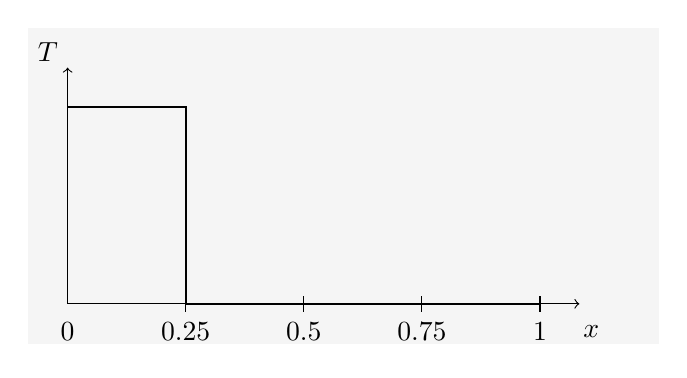
\begin{tikzpicture}
\draw[fill=gray!8,gray!8](0,0) rectangle (8,4);
%\draw[step=0.5cm,gray,very thin] (0,0) grid (8,4); %background grid

\draw[->] (0.5,0.5) -- (7,0.5) ; 
\node[] at (0.5,0.15) {$0$};

\node[] at (2,0.15) {$0.25$};
\node[] at (3.5,0.15) {$0.5$};
\node[] at (5,0.15) {$0.75$};
\node[] at (6.5,0.15) {$1$};
\draw[->] (0.5,0.5) -- (0.5,3.5) ; 
\node[] at (0.25,3.7) {$T$};


\draw[-] (2,0.4) -- (2,0.6) ; 
\draw[-] (3.5,0.4) -- (3.5,0.6) ; 
\draw[-] (5,0.4) -- (5,0.6) ; 
\draw[-] (6.5,0.4) -- (6.5,0.6) ; 


%\draw[-] (2,1) -- (1.75,0.75) ; 
%\draw[-] (2.5,1) -- (2.25,0.75) ; 
%\draw[-] (3,1) -- (2.75,0.75) ; 
%\draw[-] (3.5,1) -- (3.25,0.75) ; 
%\draw[-] (4,1) -- (3.75,0.75) ; 
%\draw[-] (4.5,1) -- (4.25,0.75) ; 

%---------------------------------

%\draw[thick,->] (7,1) -- (7,5) ; 
%\node[] at (6.6,4) {$L_y$};
%\node[] at (6.6,1) {$0$};
%\draw[-] (6.85,1) -- (7.15,1) ; 
%\draw[-] (6.85,4) -- (7.15,4) ; 
%\node[] at (7.6,4) {$p=0$};
%\node[] at (6.6,5) {$y$};

%---------------------------------

\draw[thick] (0.5,3) -- (2,3) -- (2,0.5) -- (6.5,0.5) ; 
\node[] at (7.15,0.15) {$x$};


\end{tikzpicture}



\end{center}

Set $\rho=C_p=1$.
Run the model for 250 time steps with $\delta t=0.002$.
Implement a fully implicit, explicit and Crank-Nicolson 
time discretisation. 

When using Crank-Nicolson, you should then be able to recover the green line of the 
following figure:
\begin{center}
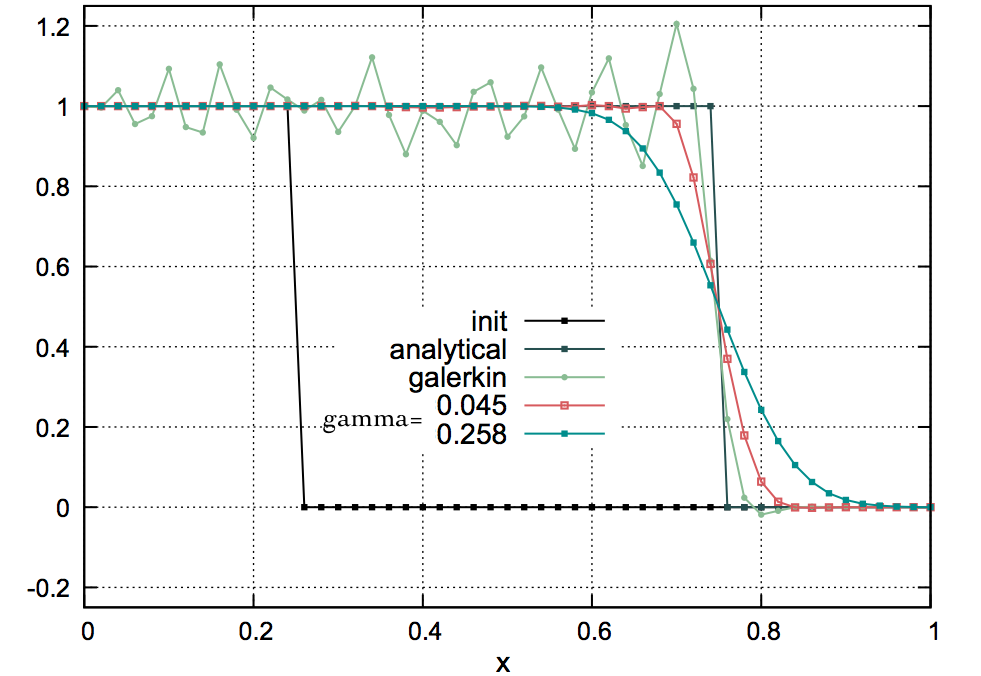
\includegraphics[width=8cm]{images/fem_exercises/fantom3.png} \\
{\captionfont Taken from Thieulot (2011) \cite{thie11}. Note that $\tau=\gamma h/u$.}
\end{center}

Finally, implement the SUPG method and recover the red and turquoise lines.

\par\noindent\rule{\textwidth}{0.4pt}
\end{minipage}
\end{center}
%-/-/-/-/-/-/-/-/-/-/-/-/-/-/-/-/-/-/











